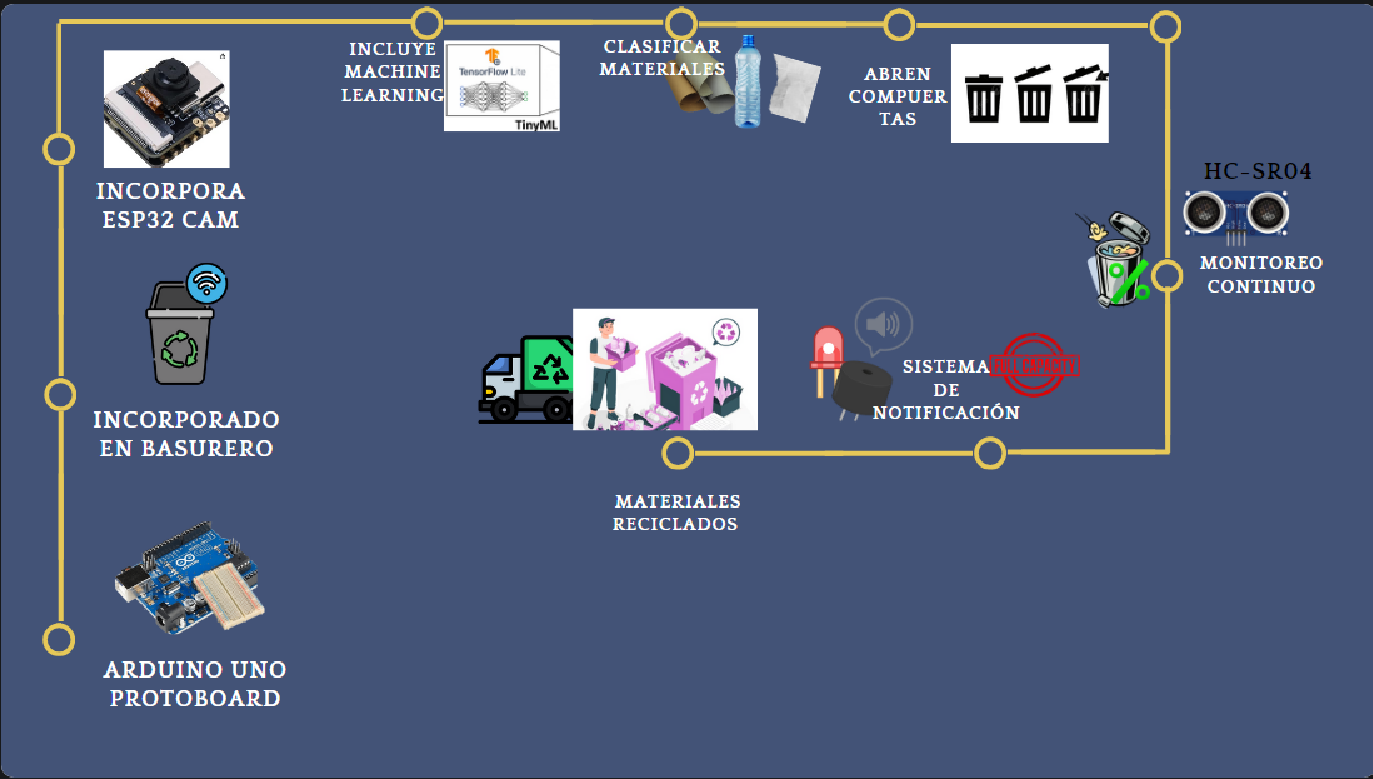
\includepdf{Imagenes/dc1.pdf}
\subsection{Descripción del diseño conceptual planteado}
\textbf{1. Arduino UNO R3}

El Arduino Uno es el corazón del sistema, encargado de recibir señales de los distintos componentes (cámara, sensores, etc.) y tomar decisiones en función de los datos recibidos.

Interacción: El Arduino coordina todo el sistema. Recibe las imágenes desde la cámara (ESP32 CAM), los datos de clasificación del modelo de machine learning (TinyML), y las lecturas del sensor ultrasónico (HC-SR04). Luego, controla la apertura de las compuertas y activa el sistema de notificación según sea necesario.

Acción: Procesa todas las señales y ejecuta comandos para manejar los actuadores y sensores.

\textbf{2. Incorporación de ESP32 CAM (Cámara)} 

La ESP32 CAM está instalada dentro del basurero. Su principal tarea es capturar imágenes de los residuos que se introducen. 

	\textbf{Interacción:} Cada vez que se coloca un objeto en el basurero, se activa la cámara para tomar una foto. Esta imagen es esencial para el siguiente paso, que es la clasificación mediante machine learning. 

	\textbf{3. Procesamiento con Machine Learning (TinyML)} 

Una vez que la cámara toma la imagen del residuo, esta se envía al sistema de machine learning, específicamente utilizando TensorFlow Lite, una versión ligera diseñada para dispositivos como la ESP32. 

    \textbf{Interacción:} El sistema de machine learning procesa la imagen en tiempo real y clasifica el material como plástico, papel, vidrio, etc. Esto se basa en el entrenamiento previo de un modelo que ha aprendido a identificar diferentes tipos de residuos. 

	\textbf{Decisión:} Dependiendo de la clasificación del material, el sistema decide en qué compartimiento debe depositarse el residuo. 

A continuación planteamos el siguiente diseño de como el modulo ESP32 CAM está involucrado de cierto modo con el proceso de machine Learning:


\begin{figure}[H]
	\centering
	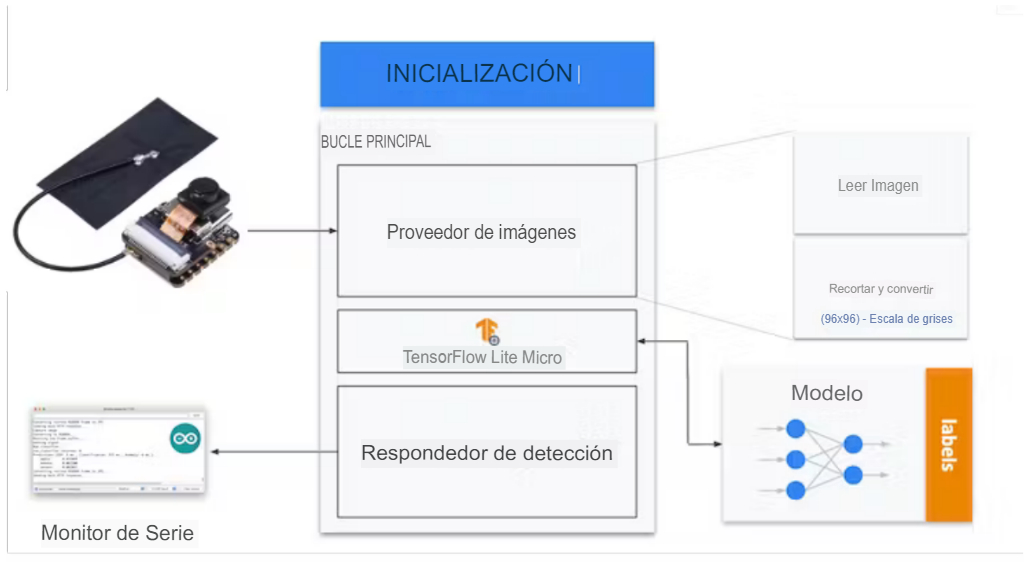
\includegraphics[scale  = 0.50]{Imagenes/ESP32-XIAO-CNN.jpg}
	\caption{ESP32 CAM y Machine Learning}{Fuente: Adaptado de~\cite{art_Xiao}}

\end{figure}

\textbf{Descripción}

\textbf{Inicialización}

Basicamente es configurar el sistema, inicializando todos los componentes del hardware y el software necesarios para realizar el procesamiento de imágenes y la clasificación.

Luego se inicializa la XIAO ESP32 CAM y el modelo de TensorFlow Lite Micro se carga en la memoria.

\textbf{Proveedor de Imágenes}

Función: La XIAO ESP32 CAM captura la imagen del objeto o material que se desea clasificar.

Proceso:

Cuando se le da una imagen a la cámara, su principal tarea es capturar la imagen y enviarla para ser procesada.

Leer Imagen: Se obtiene la imagen capturada en bruto.

Recortar y Convertir: Esta imagen es procesada, recortada y convertida a escala de grises para reducir la cantidad de datos y permitir una clasificación más eficiente. Aquí se menciona que la imagen se ajusta a una resolución de 96x96 píxeles.

\textbf{TensorFlow Lite Micro}

Función: Una vez que la imagen ha sido preprocesada, es enviada al módulo de TensorFlow Lite Micro, que está ejecutándose en la ESP32. Este módulo es responsable de aplicar el modelo de machine learning a la imagen procesada.

Proceso:
La imagen recortada y convertida es alimentada al modelo entrenado que reside en el sistema. Este modelo ha sido previamente entrenado para identificar ciertos patrones en las imágenes (clasificación de materiales, por ejemplo).

Modelo: El modelo de machine learning es una red neuronal simple, optimizada para sistemas embebidos con bajos recursos como la ESP32. El modelo toma como entrada la imagen convertida y devuelve una clasificación, basada en etiquetas predefinidas (labels) que corresponden a los materiales o categorías que el sistema debe reconocer.

\textbf{Respondedor de Detección}

Función: Una vez que el modelo ha procesado la imagen y ha generado una salida, el respondedor de detección se encarga de interpretar esta salida y tomar una acción en función de la predicción.

Proceso:
El sistema compara la salida del modelo con las etiquetas posibles (plástico, papel y cartón).

La respuesta de la detección (la etiqueta del material identificado) se envía al monitor serie para que podamos visualizarla.
Esto lo vamos a hacer por motivos de ver como se va comportando el modelo de detección y en base a eso, hacer ajustes o aplicar técnicas de optimizar.


El Arduino cuando lo conectemos puede utilizar esta salida para realizar una acción, como activar un motor para mover el residuo al compartimiento correspondiente o encender una señal de alerta.

\textbf{Monitor de Serie (Interfaz de Usuario)}

Función: El monitor de serie muestra las salidas del sistema, permitiendonos ver la clasificación en tiempo real.

Proceso:
A través de la consola de monitor serial, se pueden ver las etiquetas o categorías de los materiales clasificados.

Este componente puede también actuar como una herramienta de depuración, ayudando a entender cómo está funcionando el proceso en general.


	\textbf{4. Apertura de compuertas según la clasificación} 

Una vez que el machine learning ha clasificado el residuo, el sistema de control que viene siendo Arduino recibe la instrucción de abrir la compuerta correspondiente. 

    \textbf{Interacción:} El Arduino Uno controla motores o actuadores que abren las compuertas del basurero según el tipo de material identificado. Por ejemplo, si se detecta plástico, se abre la compuerta destinada para plásticos. 

	\textbf{Acción:} El residuo es depositado en el compartimiento adecuado para su recolección posterior. 

	\textbf{5. Monitoreo continuo del nivel de llenado (HC-SR04)} 

Mientras los residuos se van acumulando, el sensor ultrasónico HC-SR04 monitorea continuamente el nivel de llenado de cada compartimiento. 

    \textbf{Interacción:} Este sensor mide la distancia entre el residuo más alto y el sensor, que está colocado en la parte superior del compartimiento. A medida que los residuos se acumulan, el sensor detecta que la distancia se reduce, lo que indica que el compartimiento se está llenando. 

	\textbf{Decisión que va a tomar} Si el compartimiento alcanza un cierto nivel como "lleno", el sistema activará una alerta para indicar que se necesita vaciar el compartimiento(s). 

	\textbf{6. Sistema de notificación} 

El sistema incluye un mecanismo de notificación visual y/o sonora (buzzer y LEDs). Este se activa en dos situaciones principales: 

    \textbf{Llenado del compartimiento:} Cuando el sensor HC-SR04 detecta que un compartimiento está lleno, activa una señal para notificar que el basurero necesita ser vaciado. 

	\textbf{Error o evento inusual:} También puede notificar si se detecta algún material que no puede clasificarse, o si hay algún error en el proceso. 

	\textbf{Interacción:} El Arduino Uno controla las luces LED o el buzzer, emitiendo una alerta visual (como encender una luz roja) o sonora (emitir un pitido) cuando es necesario. 

	\textbf{7. Materiales reciclados y gestión de residuos} 

Los residuos clasificados correctamente son depositados en diferentes compartimientos dentro del basurero. 

    \textbf{Interacción:} Una vez que el material se clasifica y se deposita, el sistema de monitoreo continúa supervisando los niveles de llenado. Los materiales reciclados se almacenan hasta que un operador recoja los residuos para su tratamiento en una planta de reciclaje. 

	\newpage